\documentclass[10pt,letterpaper]{article}

\usepackage{graphicx}
\usepackage[margin=1in]{geometry}
\usepackage{amsmath}
\usepackage[T1]{fontenc}
\usepackage[utf8]{inputenc}
\usepackage{authblk}
\usepackage{fancyhdr}
\usepackage{lastpage}
\usepackage[parfill]{parskip}
\usepackage{subcaption}

\pagestyle{fancyplain}

% Headers
\lhead{}
\chead{Tentative Results}
\rhead{}

% Footers
\lfoot{}
\cfoot{}
\rfoot{\footnotesize Page \thepage\ of \pageref{LastPage}}

\renewcommand{\headrulewidth}{0.0pt} % No header rule
\renewcommand{\footrulewidth}{0.4pt} % Thin footer rule

\title{Federated Consistency Simulation: \\
 Increasing Conflicts (Users) with Tick Parameter Comparison}
\date{July 13, 2016}
\author[ ]{Benjamin Bengfort}
\author[ ]{Pete Keleher}
\affil[ ]{Department of Computer Science}
\affil[ ]{University of Maryland}
\affil[ ]{\textit{\{bengfort,keleher\}@cs.umd.edu}}

\begin{document}

\maketitle

This report presents results that demonstrate the impact of increasing conflicts on replication over a wide area and a comparison of the two tick ($T$) parameter models we have identified: Bailis and Howard. Conflict was simulated by using traces that had an increasing number of users (1, 3, and 5 users). We show in these results how Federated Consistency out performs both Eventual Consistency and Raft as conflicts increase. Moreover, we take a first look at the impact of the tick parameters as they relate to the mean latency.

\textbf{Note:} These results are marked as tentative because I used a more random set of traces to get these results done. The updated results will show workloads with a more clear definition of conflicts. Moreover the wide area latencies are not in the ``realistic'' range of 64ms -- 978ms in order to actually generate results.

The results include 216 simulations with the following fixed dimensions:

\begin{itemize}
    \item Number of Users: 1, 3, and 5 users
    \item Tick Parameter Model: Bailis vs. Howard
    \item Wide Area Latency, 12 mean latencies in the range $\lambda_{\mu} = [130, 2880]$,  $\lambda_{\sigma}=50$.
    \item Replication Models: Eventual, Federated, and Raft
\end{itemize}

The $T$ parameter defines the behavior of each simulation. Raft replica election timeouts are $(T, 2T)$ and heartbeat intervals are $\frac{T} {2}$. For eventual nodes the anti-entropy delay is $\frac {T} {4}$. The two models are as follows:

\begin{itemize}
    \item Bailis: $T=10\lambda_{\mu}$
    \item Howard: $T=2(\lambda_{\mu} + 2\lambda_{\sigma})$
\end{itemize}

As shown from the results in this paper, the $T$ parameter plays a large role in defining the outcome of distributed replication. The lower the $T$ parameter, the more messages that are sent in the system. Real systems would experience clogging and bandwidth reduction. In the simulation this manifests itself as increased memory usage leading to slower simulation and analysis times as well as the possibility of the OS killing processes. Much of the work that went into producing these results was about memory safety and optimization. More details on this aspect is reported in Figure \ref{fig:memory_profiler}.

\begin{figure}[!h]
    \centering
        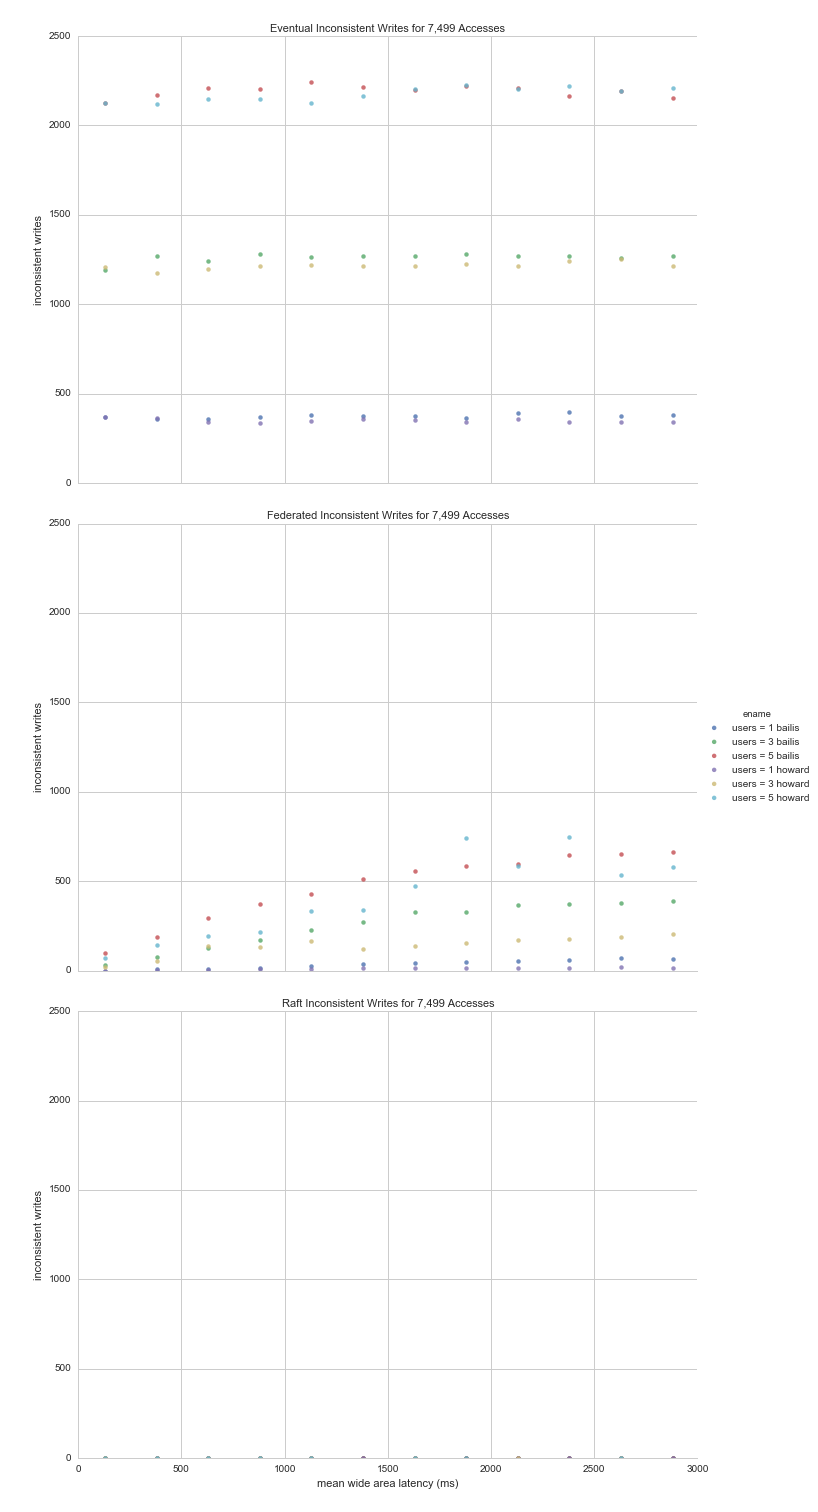
\includegraphics[height=0.9\textheight]{figures/inconsistent_writes.png}
        \caption{\textsf{Inconsistent writes are any forked writes that are written to a log. As the number of conflicts increases, so do the number of forks and therefore possible inconsistent writes. In Raft there are no inconsistent writes. There appear to be no real difference between $T$ in eventual, but in Federated, there does appear to be an increasing gap between $T$ models where Howard outperforms Bailis, except where there is so much conflict that they converge.}}
        \label{fig:inconsistent_writes}
\end{figure}

\begin{figure}[!h]
    \centering
        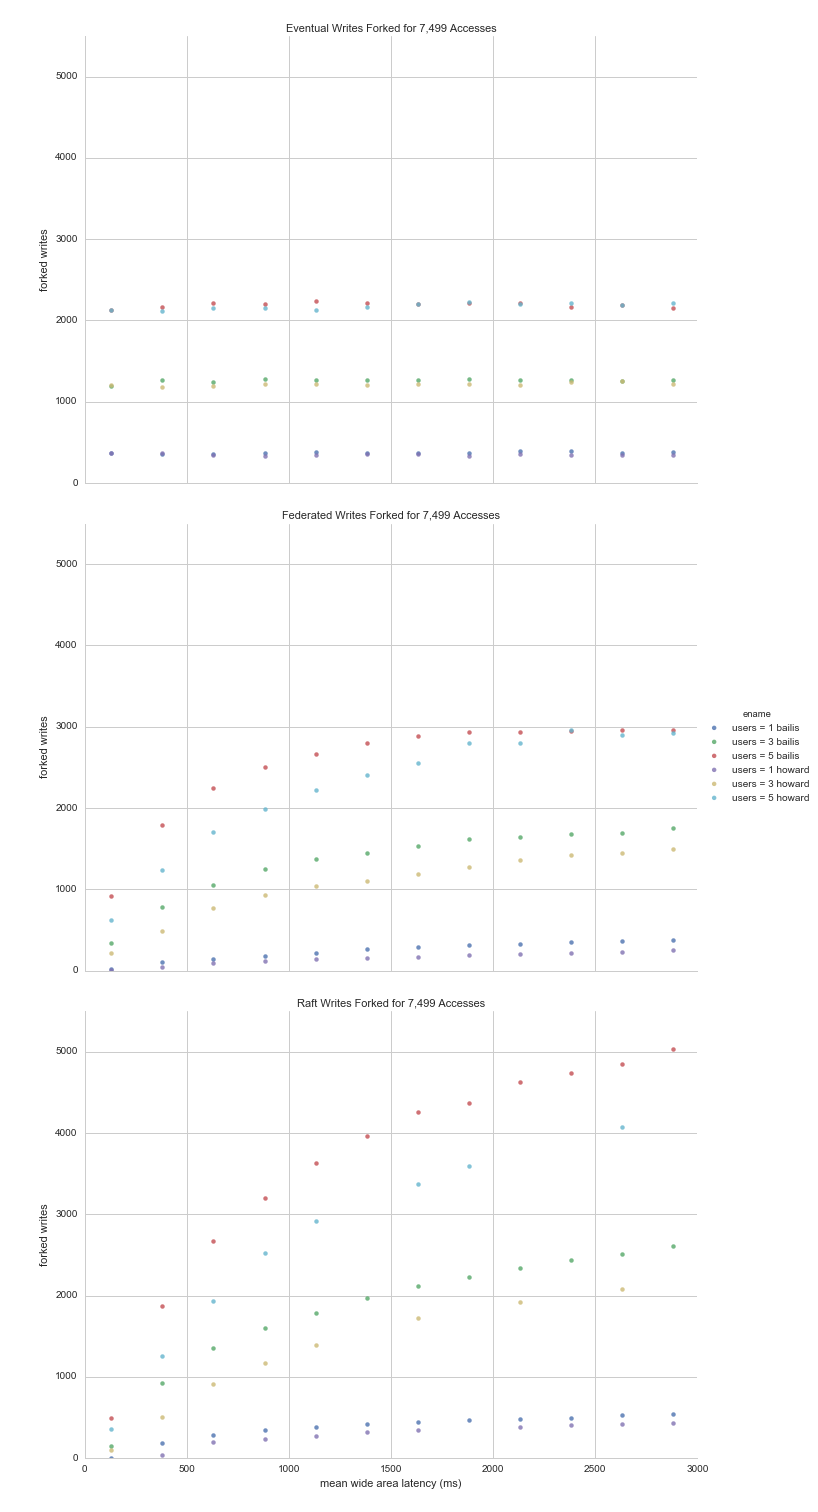
\includegraphics[height=0.9\textheight]{figures/forked_writes.png}
        \caption{\textsf{As conflict increases, so does the number of forks. For raft the $T$ parameter appears to be significant as the number of conflicts increase, but both models eventually converge as the mean latency increases. Federated consistency however shows that there is a sharp difference between Bailis and Howard, probably due to the anti-entropy interval not allowing synchronization to the strong central quorum.}}
        \label{fig:forked_writes}
\end{figure}


\begin{figure}[!h]
    \centering
        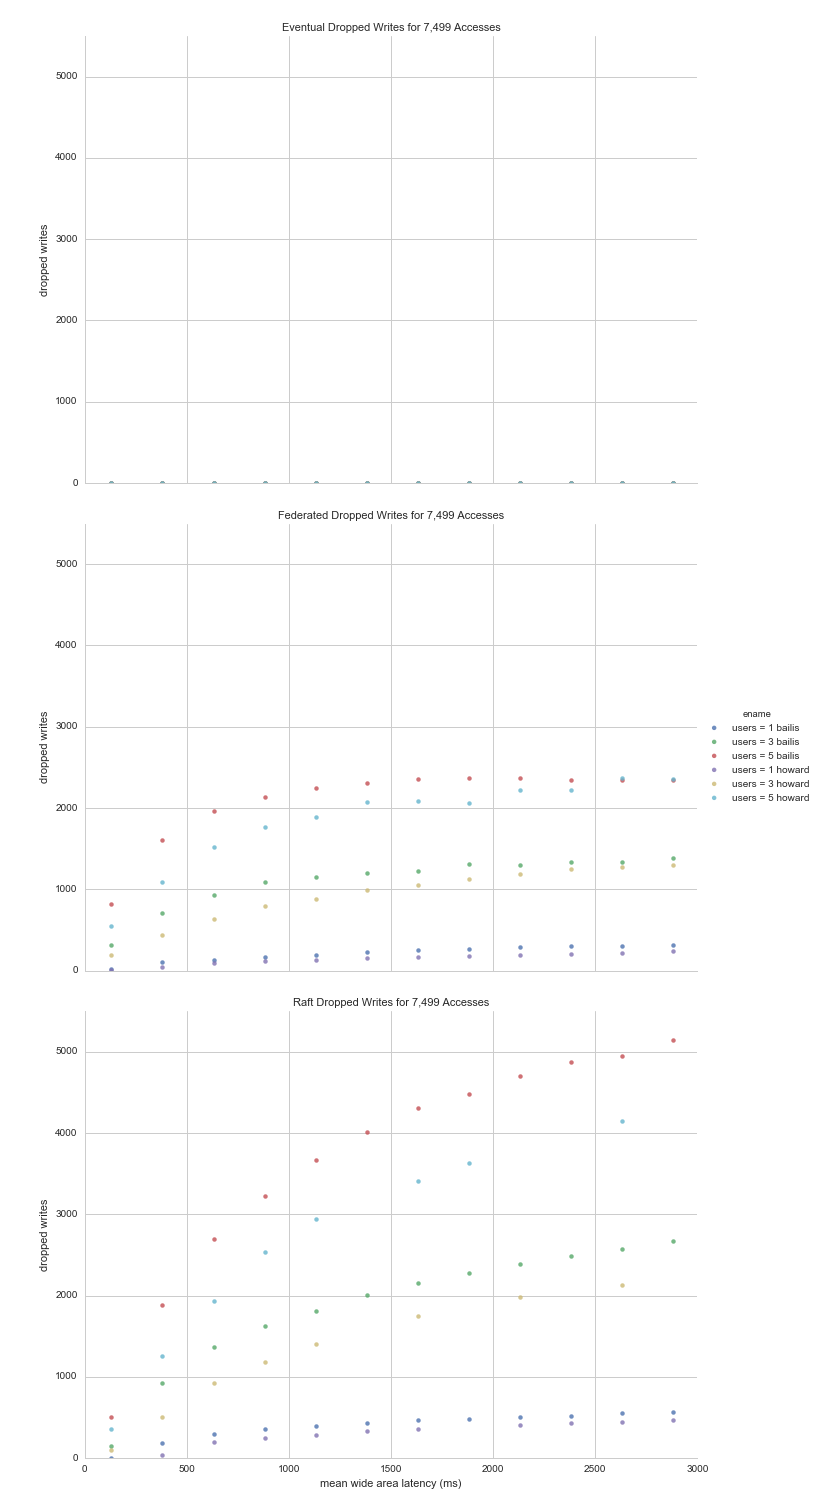
\includegraphics[height=0.9\textheight]{figures/dropped_writes.png}
        \caption{\textsf{Dropped writes is essentially the inverse of inconsistent writes in Figure \ref{fig:inconsistent_writes} and shows the same properties as the forked writes in Figure \ref{fig:forked_writes}. If eventual consistency forks writes, then Raft drops them. Federated does better by dropping some and forking other writes.}}
        \label{fig:dropped_writes}
\end{figure}

\begin{figure}[!h]
    \centering
        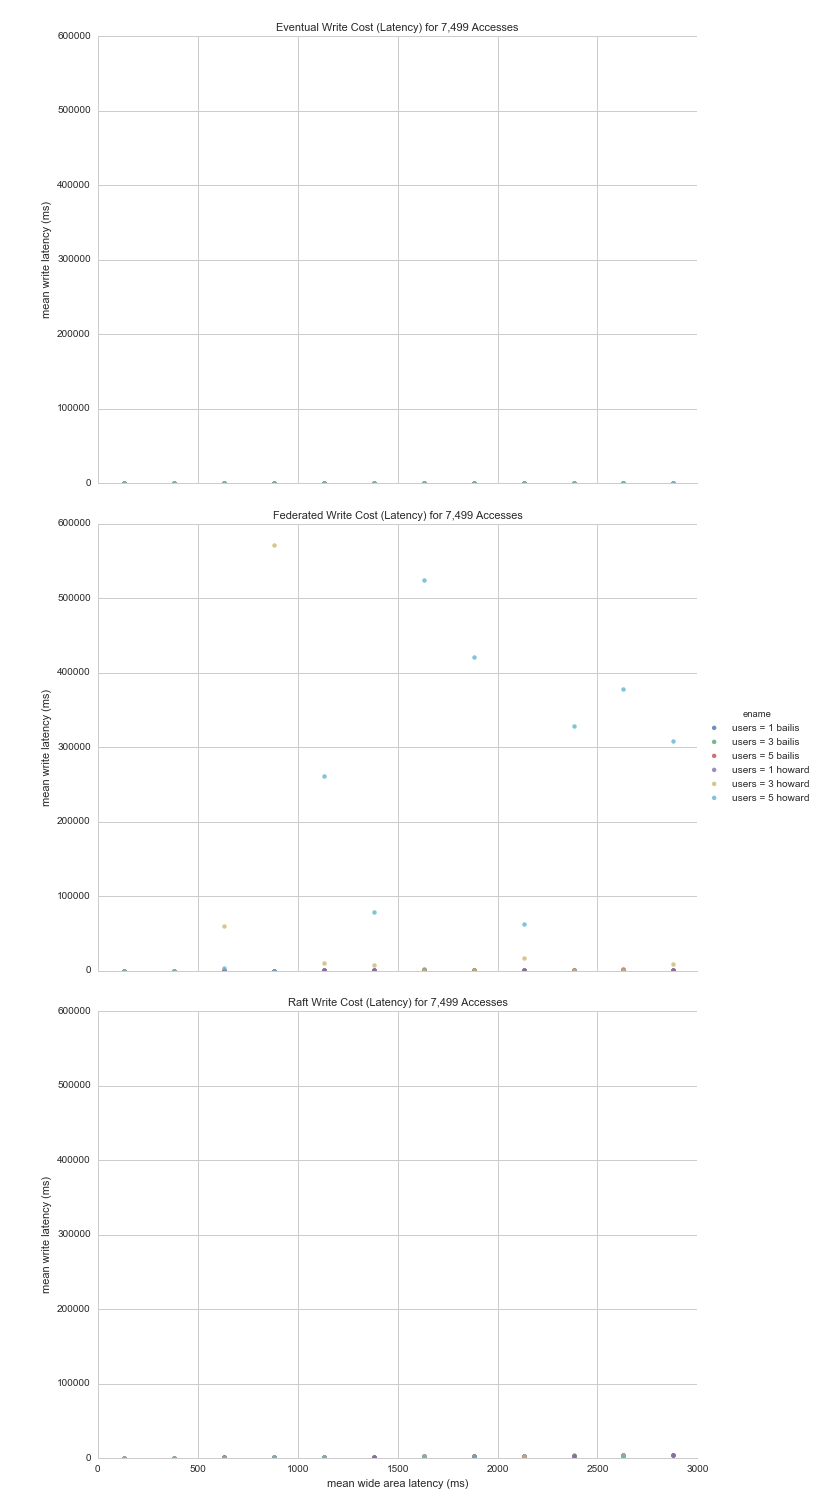
\includegraphics[height=0.9\textheight]{figures/write_latency.png}
        \caption{\textsf{This figure is all but unreadable due to the scale of the Y-Axis as a result of the write cost in Federated for the 3 and 5 user Howard models. Eventual has no write cost, and the same effect does not present itself in Raft for any model, so I believe this is a bug in the analysis - but am not sure. Potentially this is related to the cost of an remote write from an eventual node to a Raft node.}}
        \label{fig:write_latency}
\end{figure}


\begin{figure}[!h]
    \centering
        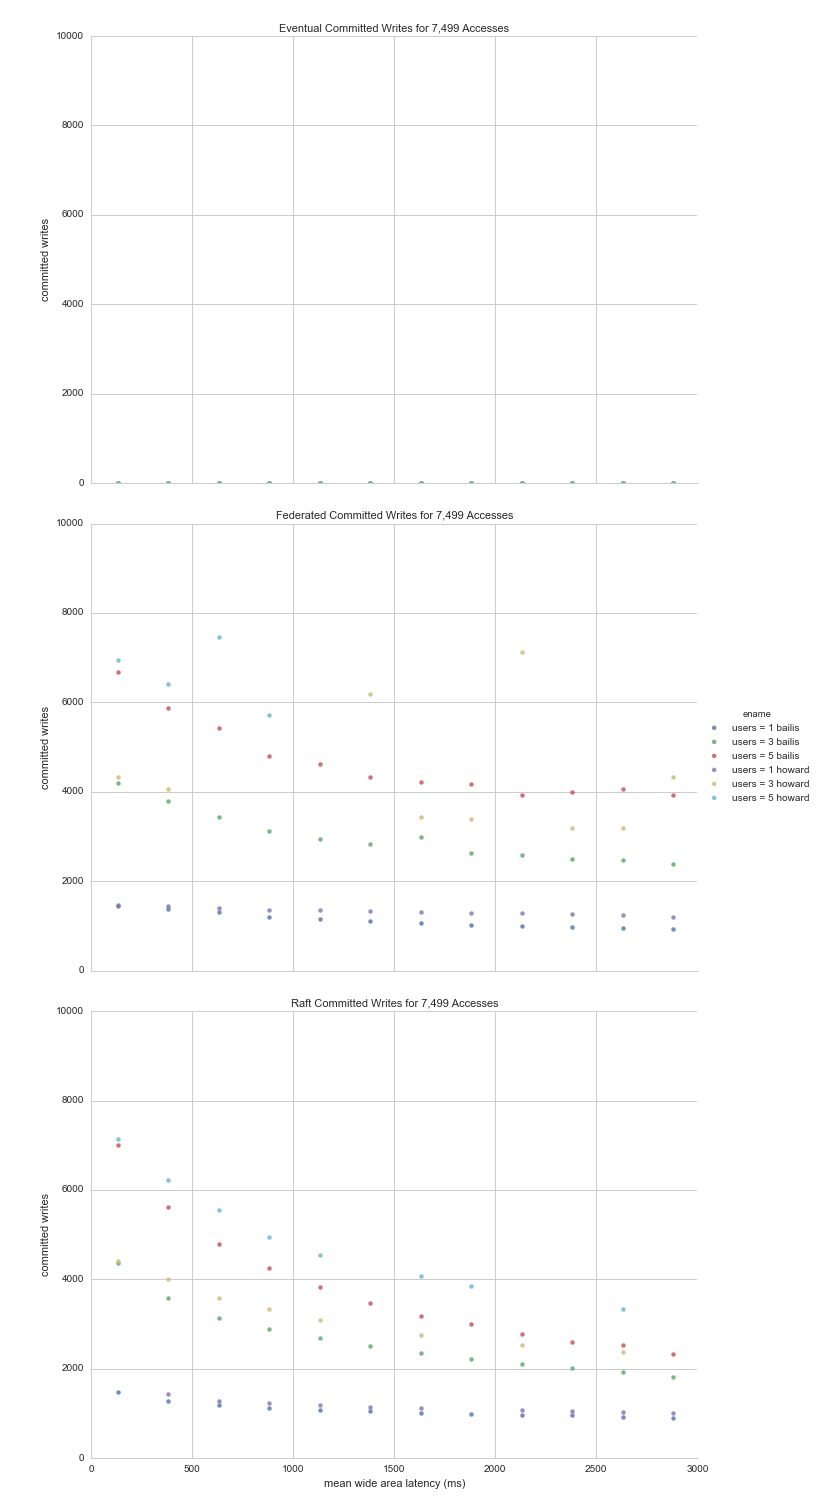
\includegraphics[height=0.9\textheight]{figures/committed_writes.png}
        \caption{\textsf{This was one of the interesting results in the last report, Federated had less writes dropped and more writes committed therefore outperformed both Raft and Eventual. There is certainly a less steep decline in commits as the wide area increases, and both $T$ models converge faster. It may also be tougher to distinguish Federated's benefits at this latency scale (as opposed to sub-second latencies).}}
        \label{fig:committed_writes}
\end{figure}

\begin{figure}[!h]
    \centering
        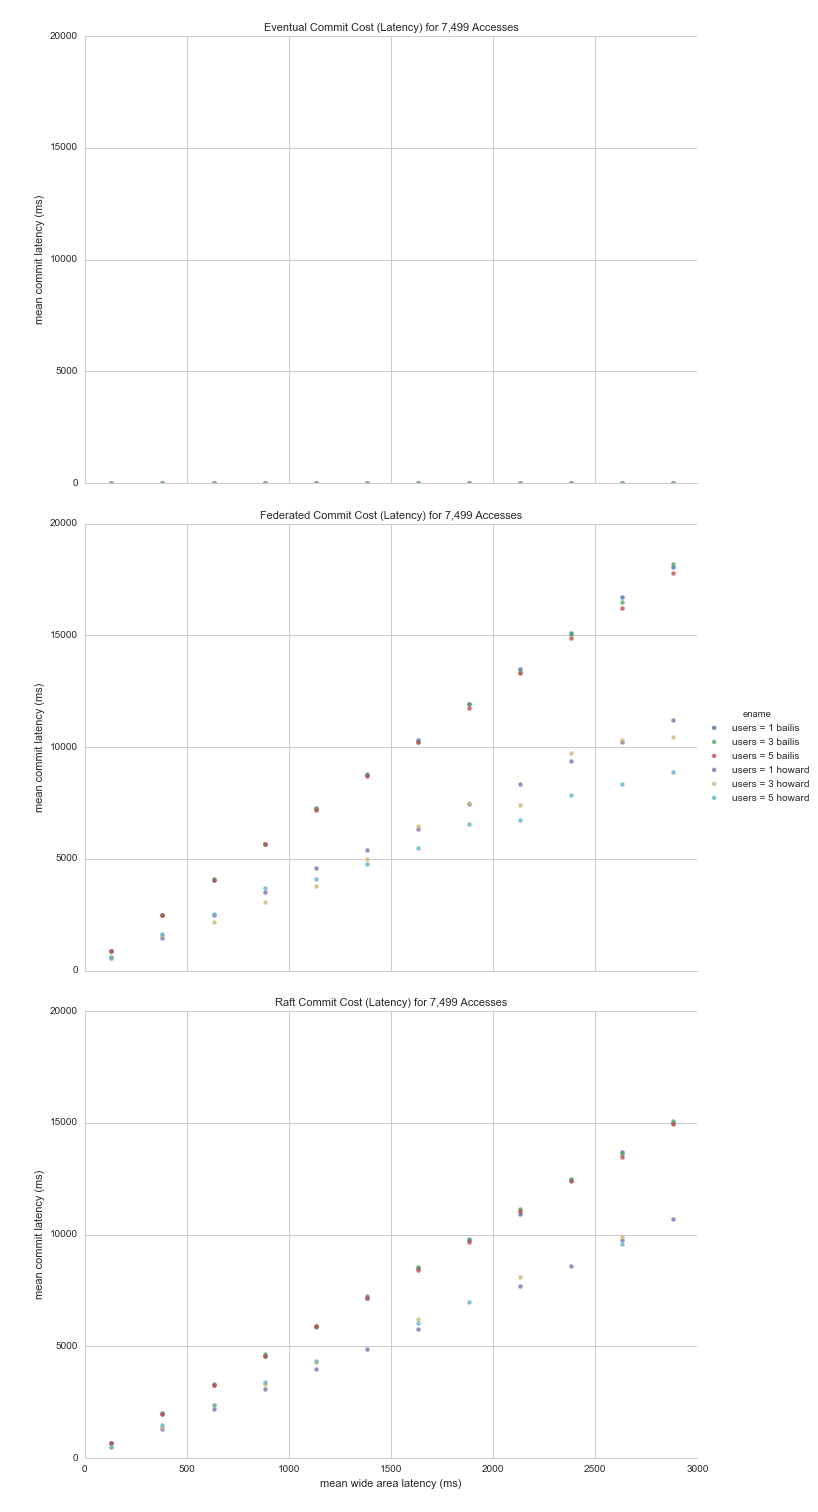
\includegraphics[height=0.9\textheight]{figures/commit_latency.png}
        \caption{\textsf{Both Raft and Federated experience a linear commit latency cost (two round trip \texttt{AppendEntries} for commit) as the mean wide area latency increases. As a result there is nearly no difference in the $T$ parameters for each set of conflicts. It is also important to note that as the number of conflicts increases, the commit cost grows steeper.}}
        \label{fig:commit_latency}
\end{figure}

\begin{figure}[!h]
    \centering
        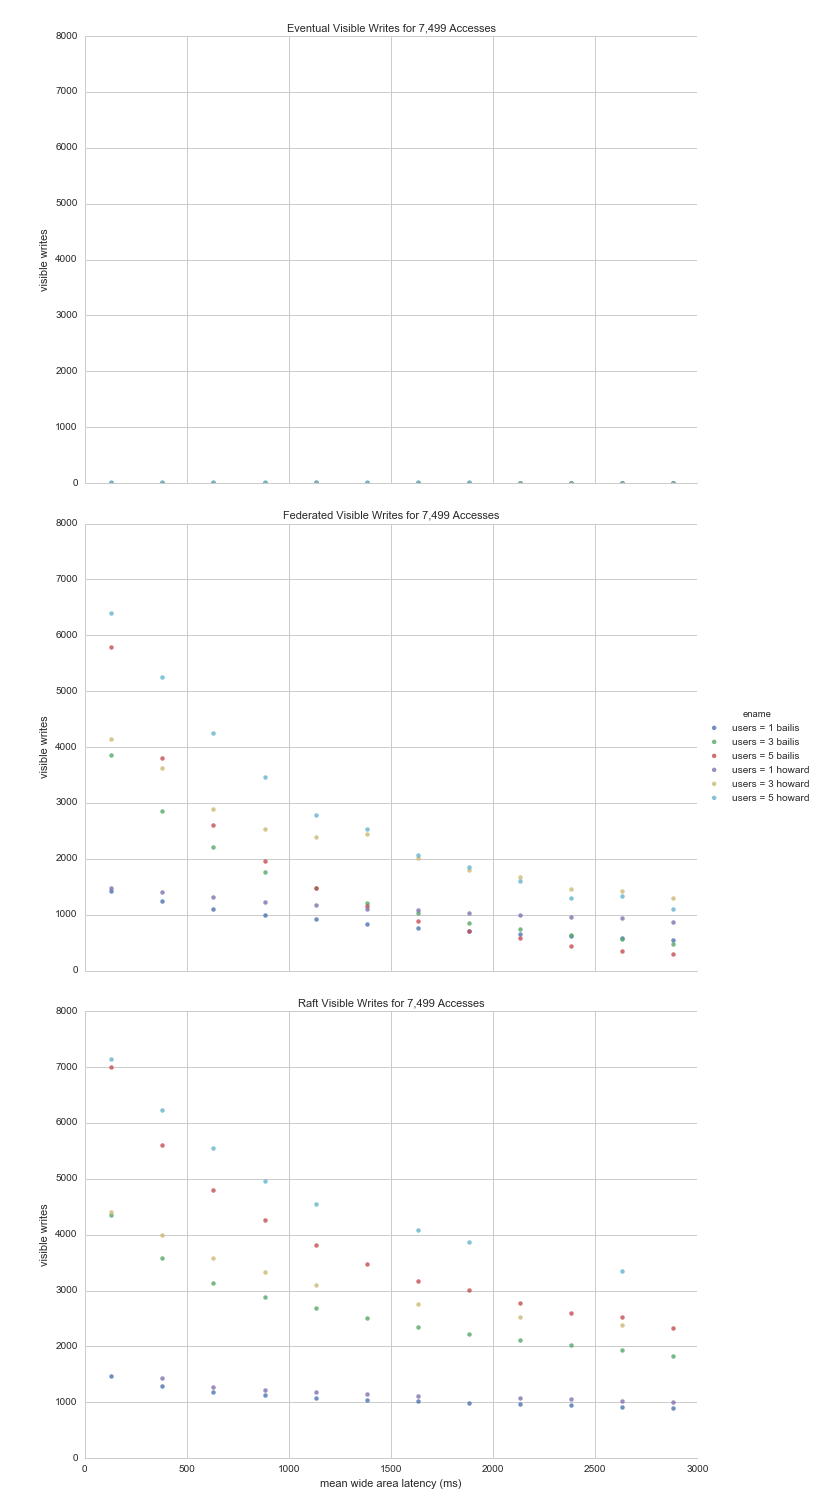
\includegraphics[height=0.9\textheight]{figures/visible_writes.png}
        \caption{\textsf{The number of writes that become visible, e.g. fully replicated. More conflict should mean that less writes become fully visible; I'm going to have to check on this graph.}}
        \label{fig:visible_writes}
\end{figure}

\begin{figure}[!h]
    \centering
        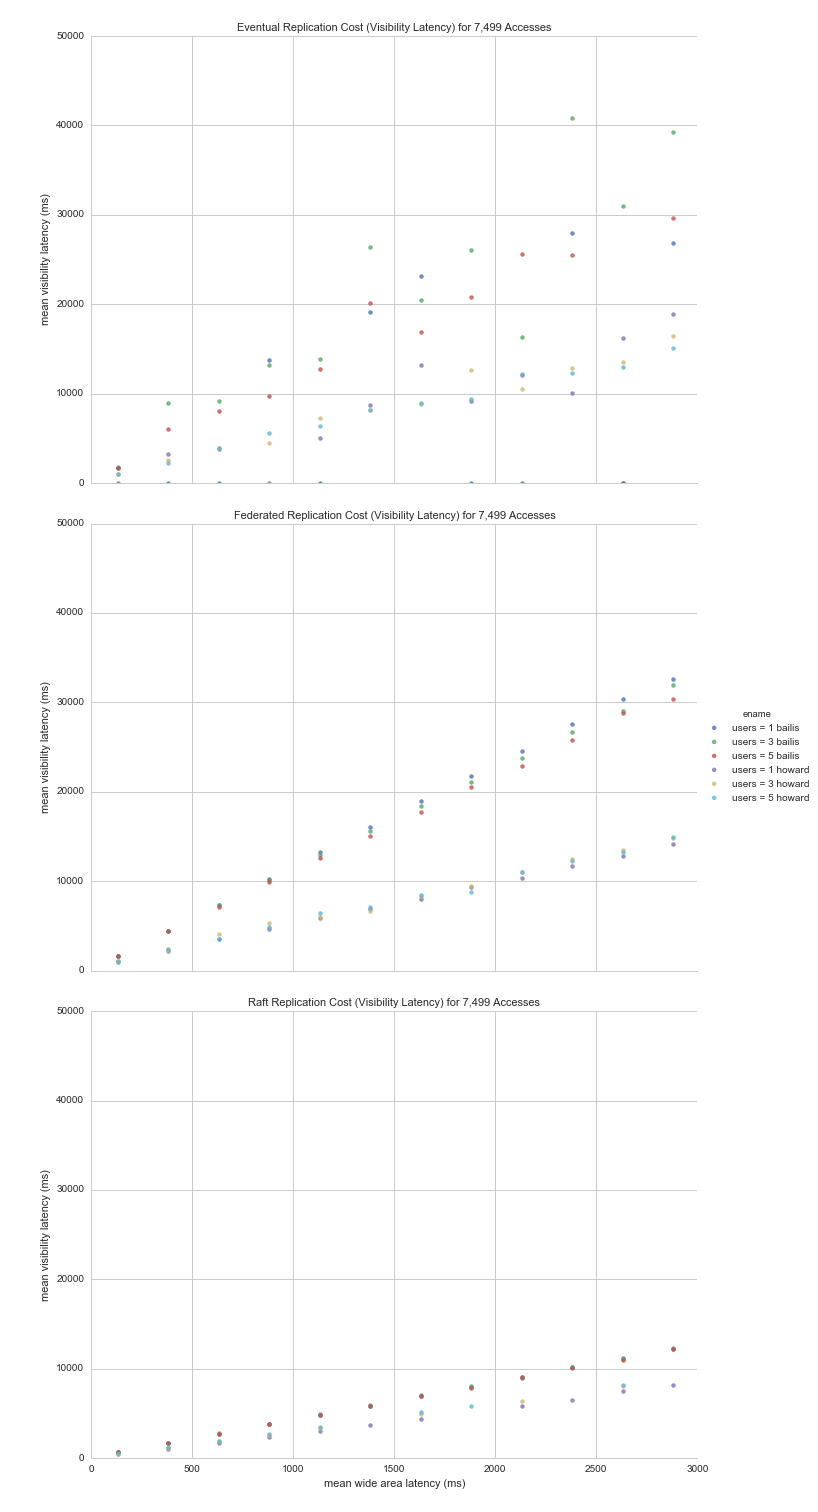
\includegraphics[height=0.9\textheight]{figures/visibility_latency.png}
        \caption{\textsf{The visibility latency is the time in ms it takes for a write to become fully visible. There is no relationship between the number of conflicts and visibility latency; however there is a clear difference between the $T$ parameter and the visibility latency, one that is widened in Federated.}}
        \label{fig:visibility_latency}
\end{figure}

\begin{figure}[!h]
    \centering
        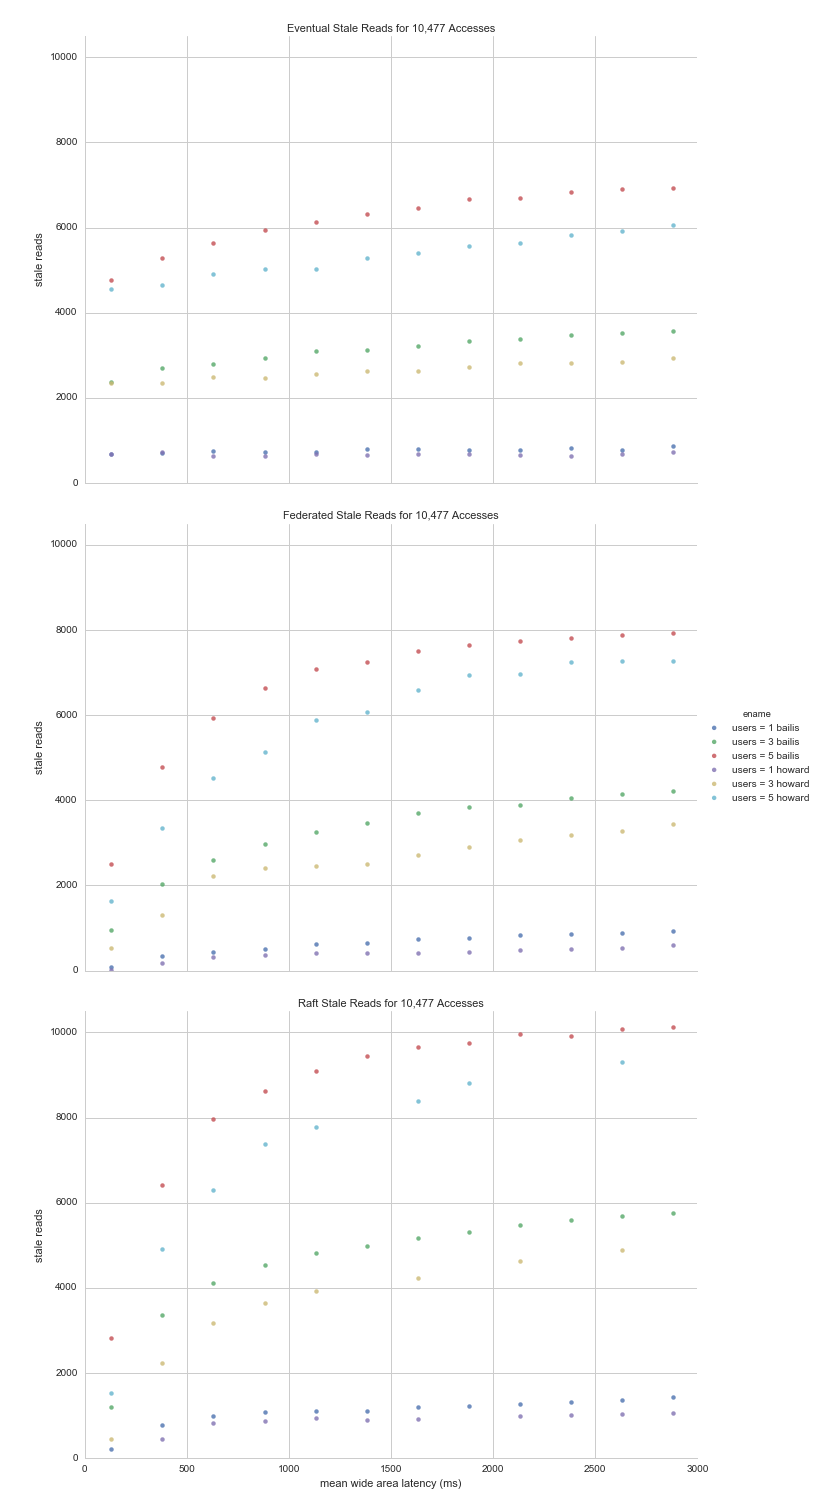
\includegraphics[height=0.9\textheight]{figures/stale_reads.png}
        \caption{\textsf{Raft has way more stale reads, and the more conflict that exists, the more stale reads there are. Howard once again outperforms Bailis.}}
        \label{fig:stale_reads}
\end{figure}

\begin{figure}[!h]
    \centering
        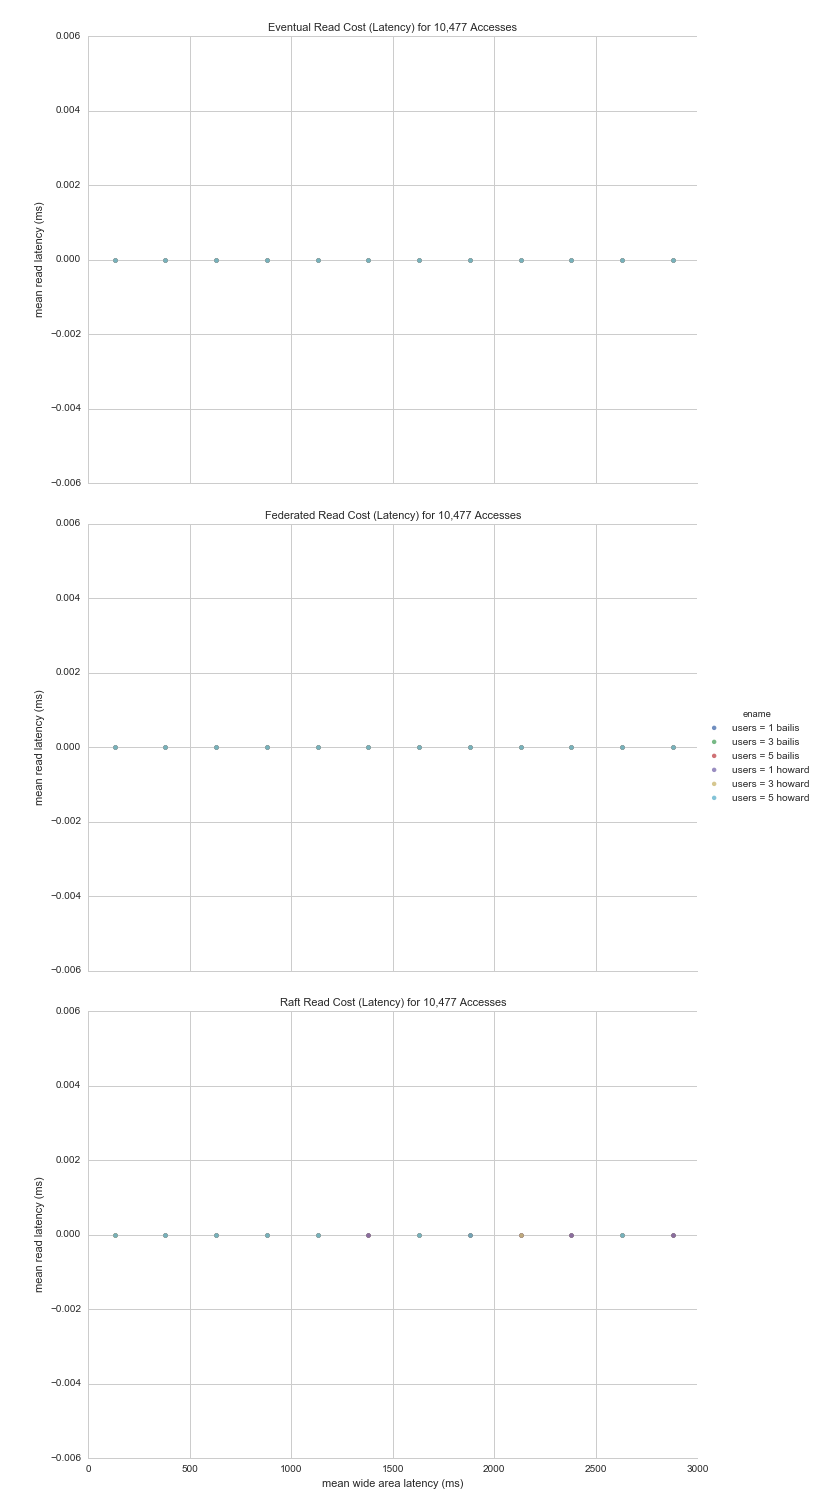
\includegraphics[height=0.9\textheight]{figures/read_latency.png}
        \caption{\textsf{There are no remote reads in this system, therefore read latency is instantaneous.}}
        \label{fig:read_latency}
\end{figure}

\begin{figure}[!h]
    \centering
        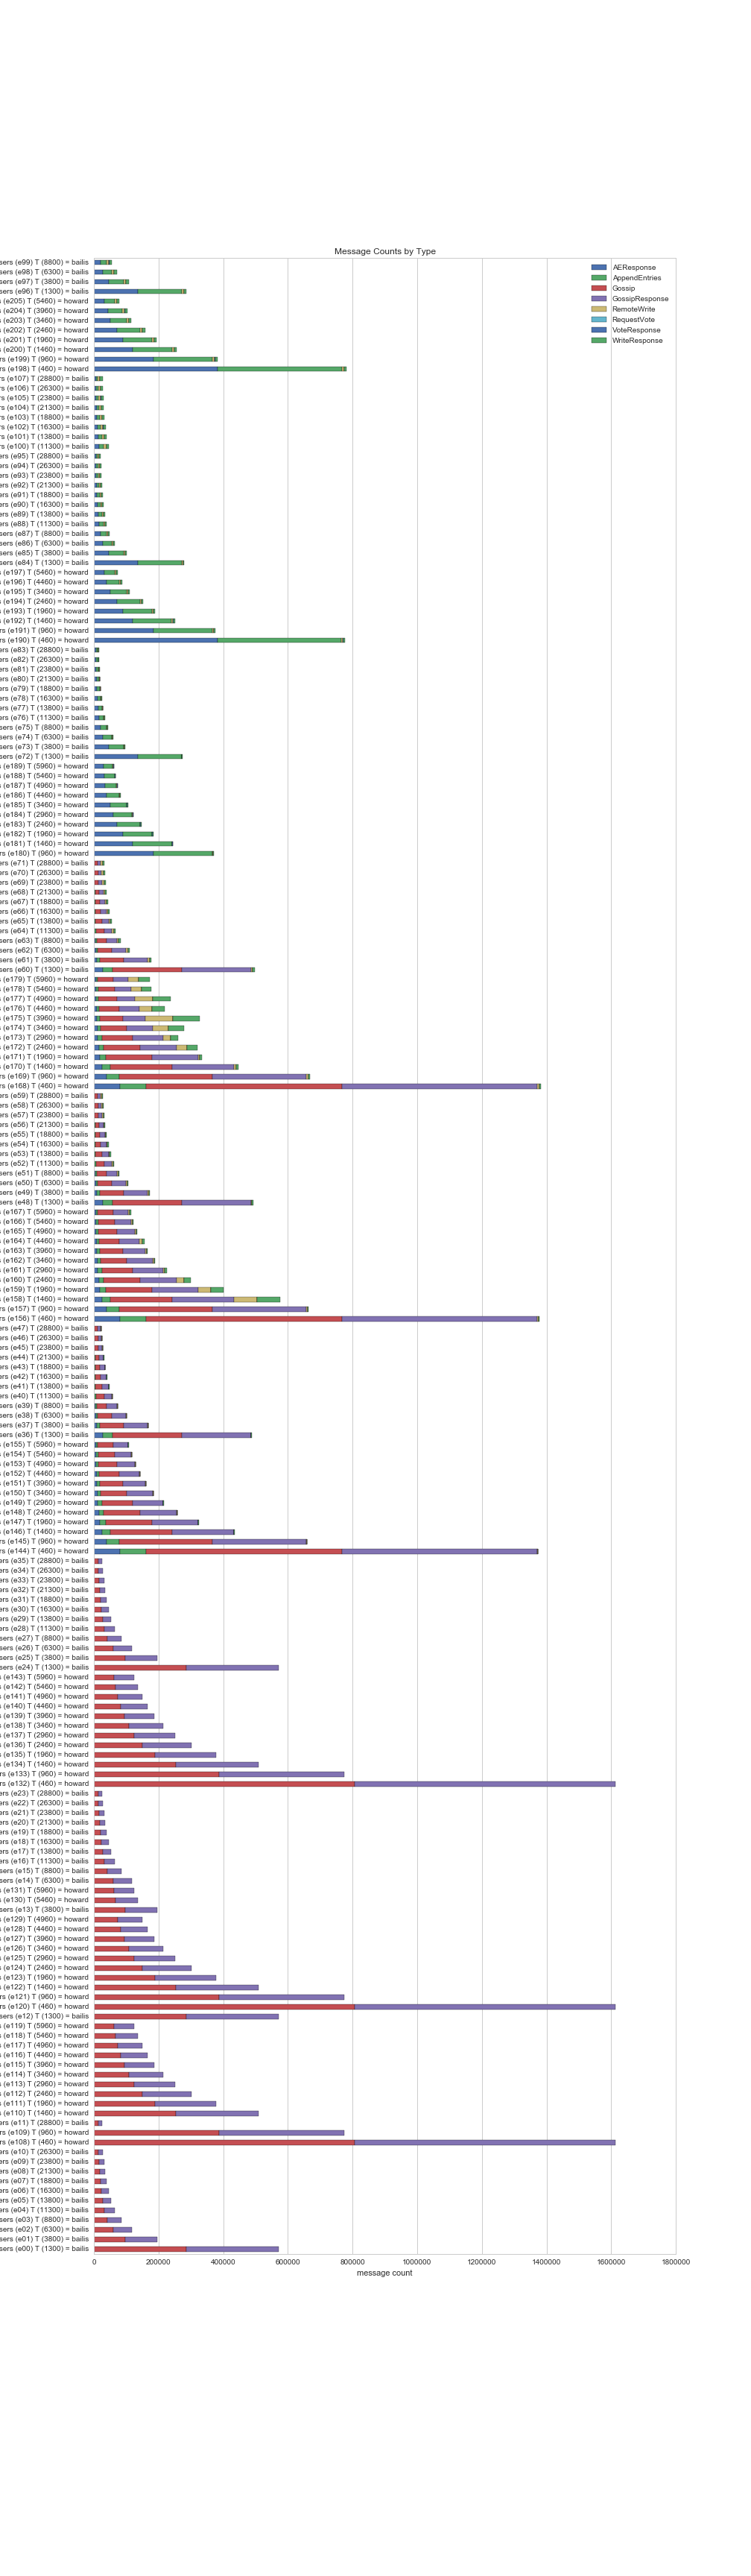
\includegraphics[height=0.9\textheight]{figures/message_counts.png}
        \caption{\textsf{The number of messages sent by a consistency model (either Raft or Eventual) is highly dependent on its timing parameters (election timeout, heartbeat interval, and anti-entropy delay). Although this graph is near unreadable, comparing the shapes of the bar charts shows that as $T$ decreases the number of messages increases, but remains generally the same for increasing number of users (only remote writes is increased). The bar chart goes 1 raft user: bailis then howard (descending $T$), then three then 5 users, then repeats for federated and eventual. }}
        \label{fig:message_counts}
\end{figure}

\begin{figure}[!h]
    \centering
        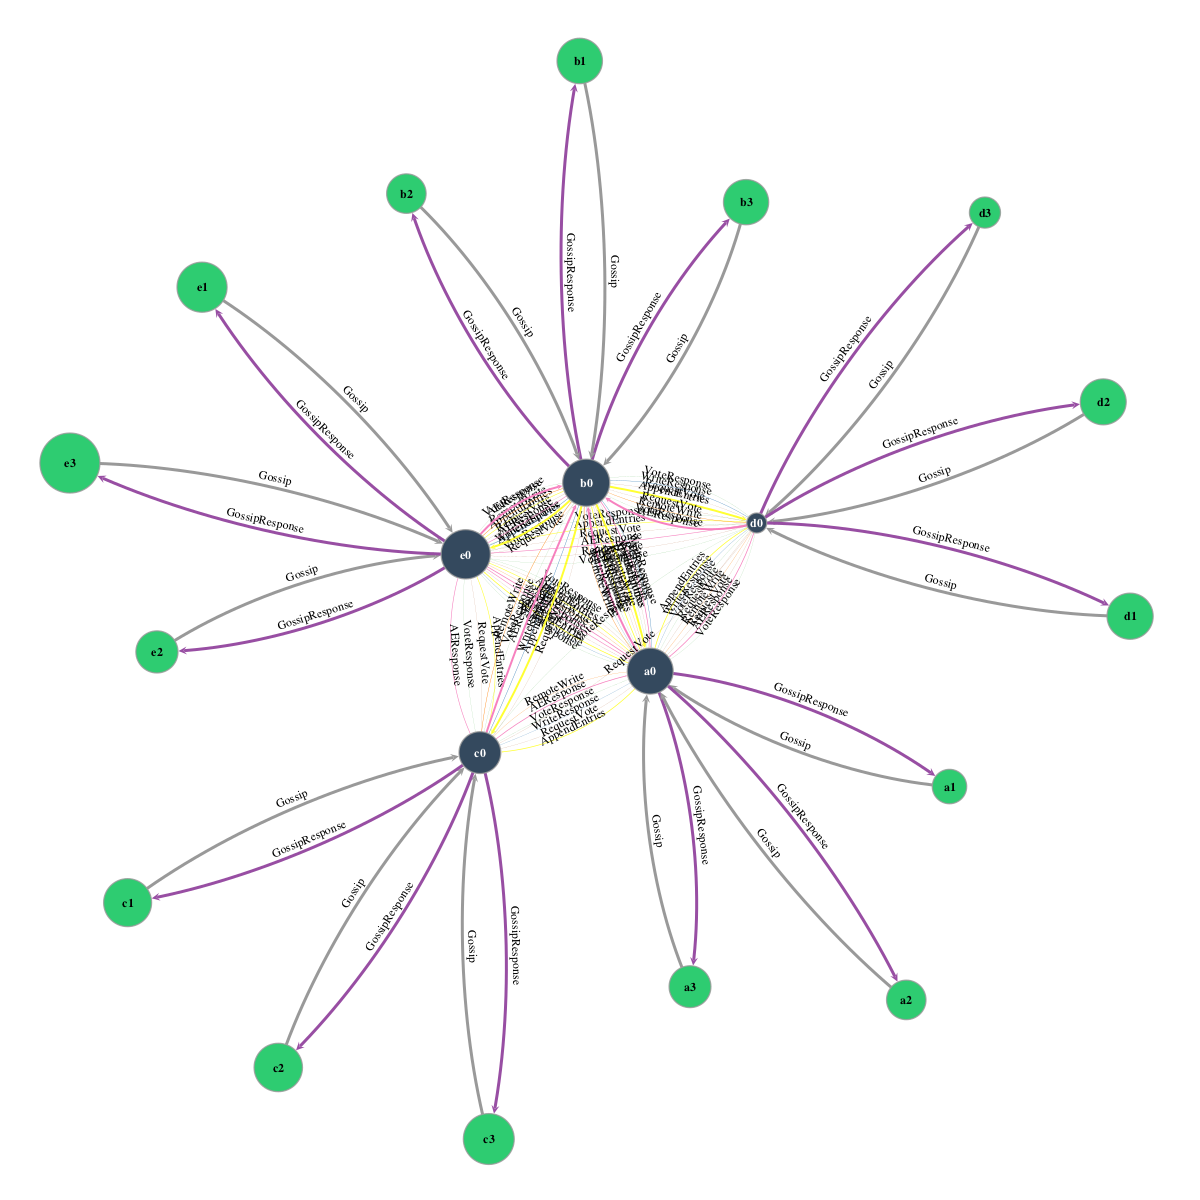
\includegraphics[width=\textwidth]{figures/federated-T460.png}
        \caption{\textsf{Network topology of the federated consistency model for 5 users and $T=460$. Edges define communication by message type (both color and label indicate the message type), message frequency between nodes is indicated by edge thickness. Vertices are colored by their consistency model (Raft and Eventual in Federated). Vertex size indicates the number of \textit{writes} that occurred at that node. The workload is fairly evenly distributed amongst the nodes.}}
        \label{fig:topology}
\end{figure}

\begin{figure}[!h]
    \centering
        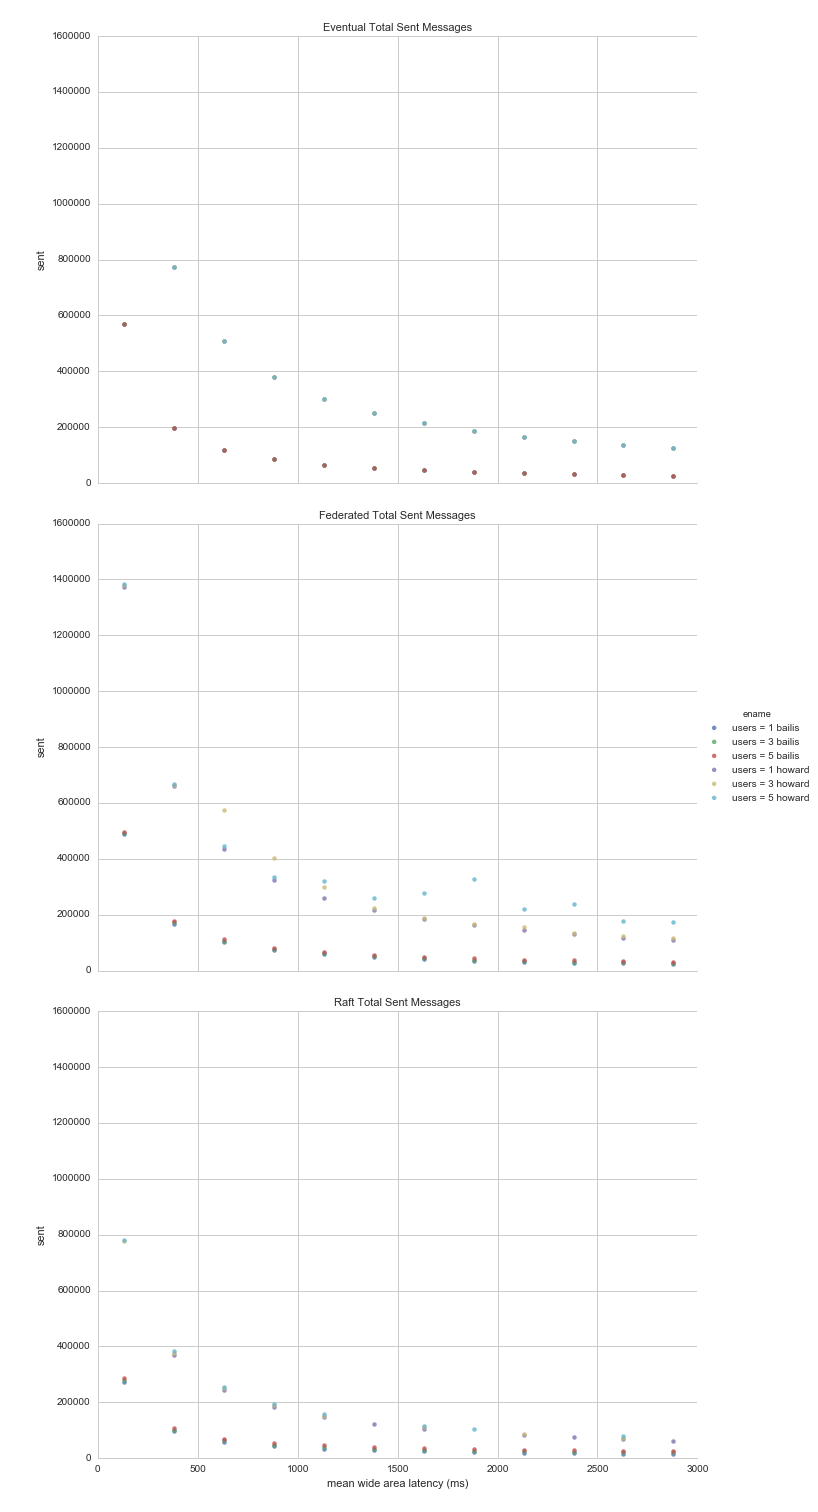
\includegraphics[height=0.9\textheight]{figures/messages_sent.png}
        \caption{\textsf{Total number of messages sent per consistency model. The lower the mean wide area latency, the lower the T, causing more messages to be sent. The number of messages is exponentially related to the mean network latency. Here the two models are basically stacked on top of each other, but the number of users doesn't make a lot of difference.}}
        \label{fig:messages_sent}
\end{figure}


\begin{figure}[!h]
    \centering
        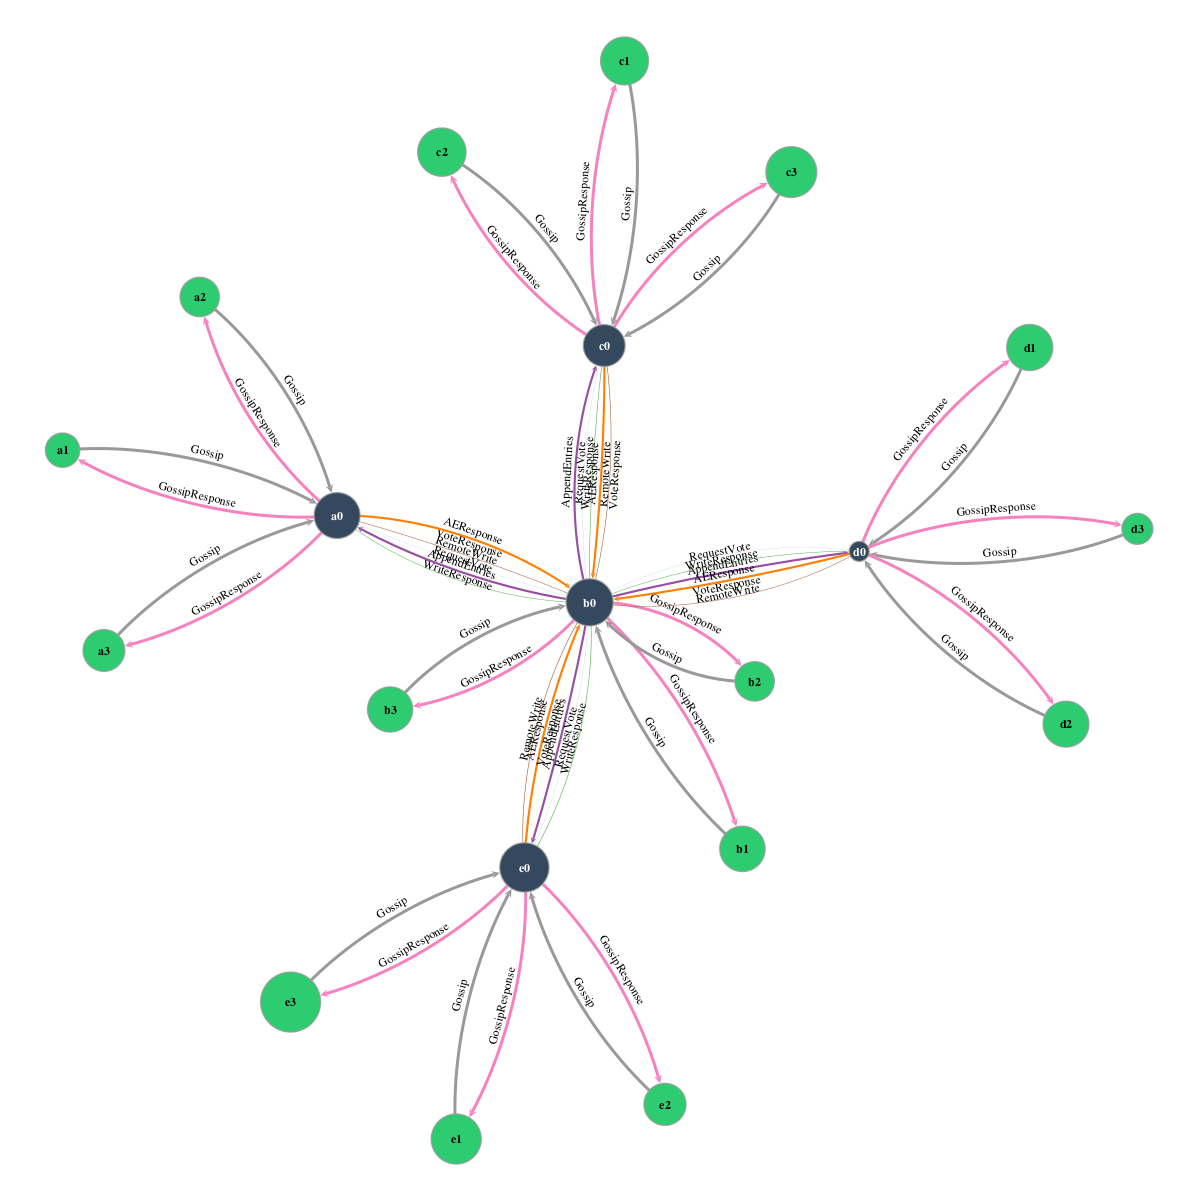
\includegraphics[width=\textwidth]{figures/federated-TNone.png}
        \caption{\textsf{Network topology of the federated consistency model for 5 users and $T=28800$. Edges define communication by message type (both color and label indicate the message type), message frequency between nodes is indicated by edge thickness. Vertices are colored by their consistency model (Raft and Eventual in Federated). Vertex size indicates the number of \textit{writes} that occurred at that node. Compared to the other network graph, this simply shows there are far less messages.}}
        \label{fig:topology}
\end{figure}

\begin{figure}[!h]
    \centering
        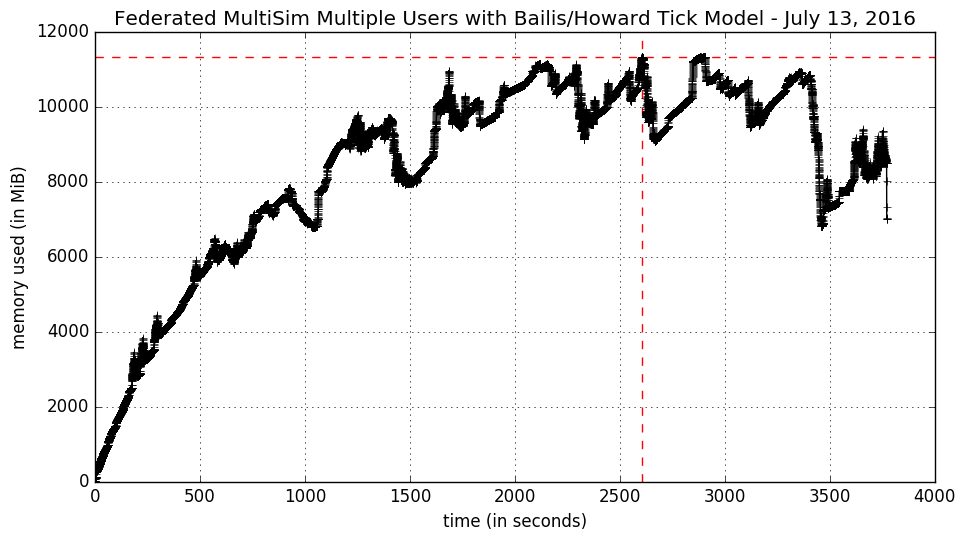
\includegraphics[width=\textwidth]{figures/memory_profiler.png}
        \caption{\textsf{The simulator ran 216 simulations with 10 errors (all Raft with low Howard parameters) in 1 hour 3 minutes via 8 parallel tasks. This figure shows the memory usage of the simulator, summing the memory of all 9 processes (master + 9 workers). I did extensive work today to reduce the amount of memory usage both in the simulator and the analysis to allow this many simulations to be inspected at once.}}
        \label{fig:memory_profiler}
\end{figure}

\end{document}
